\begin{document}
\renewcommand{\thefigure}{SI.\arabic{figure}}
\setcounter{figure}{0}

\renewcommand{\thetable}{SI.\arabic{table}}
\setcounter{table}{0}

\section*{Supplementary Information}\label{sec:SI}

\addcontentsline{toc}{section}{Supplementary Information}
\addtocontents{toc}{\setcounter{tocdepth}{-10}}
\renewcommand{\thesubsection}{SI.\arabic{subsection}}
\setcounter{subsection}{0}


\subsection{Overview}

\begin{figure}[H]
    \centering
    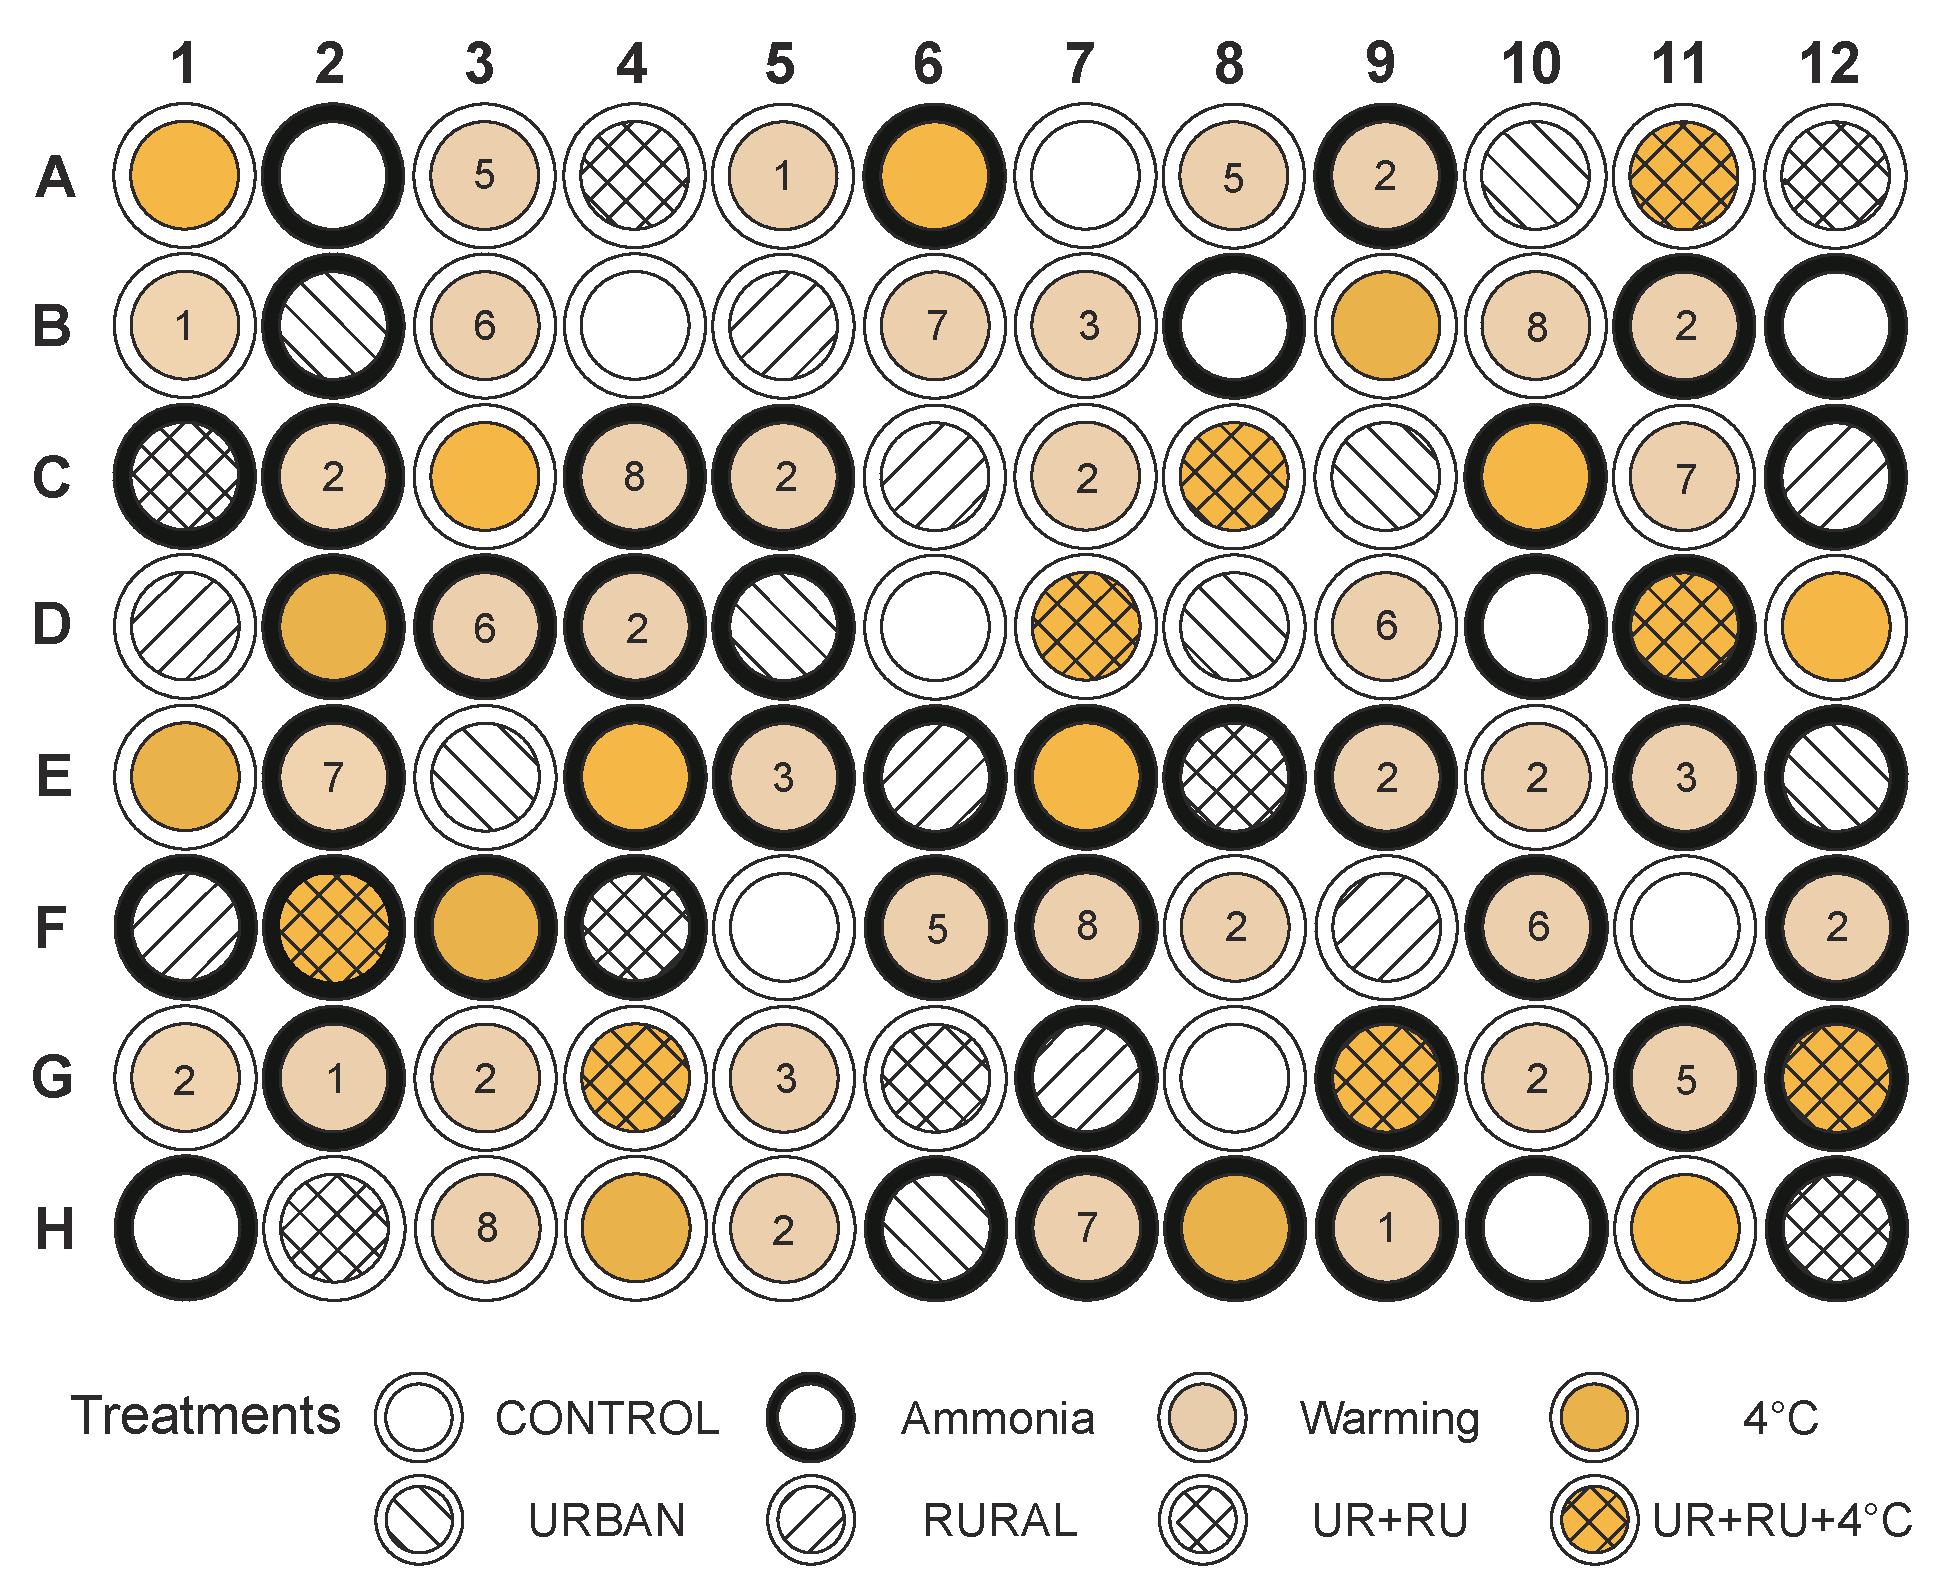
\includegraphics[scale=0.35]{./Figures/Mesocosm}
    \caption{\textbf{Treatment layout of the 96 mesocosms arranged by 8 rows of 12 individual mesocosms.} There are 12 ponds for undisturbed ambient conditions (CONTROL), 8 ponds for the URBAN, RURAL, UR+RU and UR+RU+4°C treatments respectively, and 14 ponds with a 4°C warming. Half of the mesocosms are treated with ammonia (n = 48).}
    \label{fig:Mesocosm}
\end{figure}

\begin{table}[H]
    \caption{\bf The distribution of different treatments.}
    \centering
    \begin{tabular}{ |m{6.6cm}<{\centering}|m{3.5cm}<{\centering}|m{3.5cm}<{\centering}| } 
    \hline
     Treatment & Without Ammonia & Ammonia \\
     \hline
     Control (n=12) & 6 & 6 \\ 
     +1°C (n=4) & 2 & 2 \\
     +2°C (n=14) & 7 & 7 \\
     +3°C (n=4) & 2 & 2 \\
     +4°C (n=14) & 7 & 7 \\
     +5°C (n=4) & 2 & 2 \\
     +6°C (n=4) & 2 & 2 \\
     +7°C (n=4) & 2 & 2 \\
     +8°C (n=4) & 2 & 2 \\
     Urban chemicals (n=8) & 4 & 4 \\
     Rural chemicals (n=8) & 4 & 4 \\
     Urban and rural chemicals (n=8) & 4 & 4 \\
     Urban and rural chemicals, +4°C (n=8) & 4 & 4 \\
    \hline
    \end{tabular}    
    \label{tab:Treatment}
\end{table}

\subsection{Temperature}\label{section:temp}

\begin{figure}[H]
    \centering
    \includegraphics[scale=0.85]{./Figures/Temperature/Mean_month_temp_chem}
    \caption{\textbf{Average monthly temperature of chemical treatment ponds for 2019-2022.} Deep A and B are the different locations of the temperature detectors in the pond.}
    \label{fig:mean_m_temp_chem}
\end{figure}

\begin{figure}[H]
    \centering
    \includegraphics[scale=0.84]{./Figures/Temperature/Mean_month_temp}
    \caption{\textbf{Average monthly temperature of warming treatment ponds for 2019-2022.} Deep A and B are the different locations of the temperature detectors in the pond.}
    \label{fig:mean_m_temp}
\end{figure}

\begin{figure}[H]
    \centering
    \includegraphics[scale=0.78]{./Figures/Temperature/Daily_temp_AB}
    \caption{\textbf{Average daily temperature of the warming treatment ponds for 2019-2022.} Deep A and B are the different locations of the temperature detectors in the pond.}
    \label{fig:d_tempAB}
\end{figure}

\subsection{ATP assays}\label{section:ATPsup}

\begin{figure}[H]
    \centering
    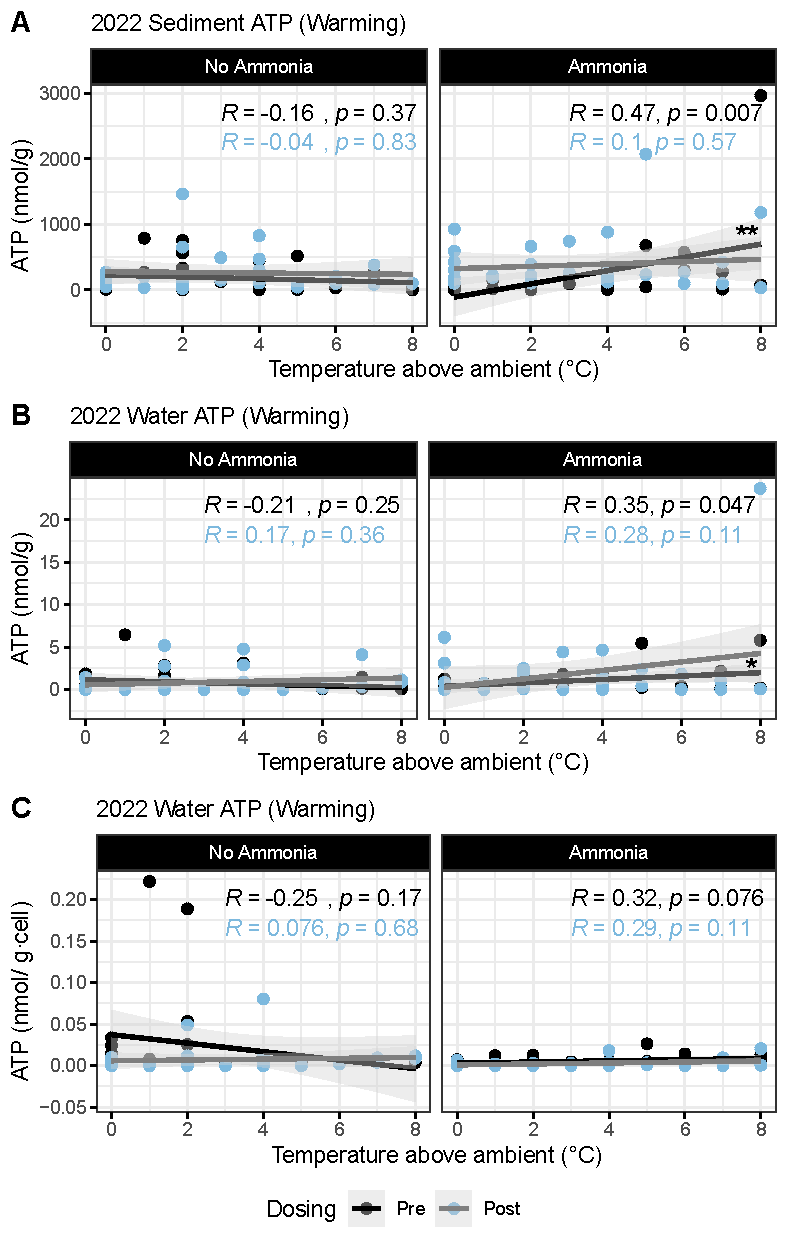
\includegraphics[scale=1]{./Figures/Regression_ATP}
    \caption{\textbf{Trends in ATP production with warming in 2022.} Before dosing, ATP production in sediment and water samples from ammonia-treated ponds increased significantly with warming. After dosing, the gradient warming did not affect ATP production significantly.}
    \label{fig:ATP2022Regression}
\end{figure}

\subsubsection{ATP production from sediment wash samples}

\begin{table}[H]
    \caption{{\bf The performance of LMM (p-values) in determining the effect of different chemical treatments on sediment wash ATP.} All treatments did not significantly affect ATP production.}
    \centering
    \begin{tabular}{ m{2.5cm}<{\centering}m{1.5cm}<{\centering}m{1.5cm}<{\centering}m{1.5cm}<{\centering}m{1.5cm}<{\centering}m{2.2cm}<{\centering}m{2.2cm}<{\centering}}
    \toprule
    Treatment & 4°C & UR & RU & UR+RU & UR+RU+4°C & Temperature \\
     \midrule
    No Ammonia & 0.904 & 0.662 & 0.848 & 0.482 & 0.873 & 0.647 \\
    Ammonia & 0.585 & 0.190 & 0.302 & 0.465 & 0.340 & 0.709 \\
    \bottomrule
    \end{tabular}    
    \label{tab:ATPSW_treat}
\end{table}

In the warming-treated ponds, only the ammonia-treated 5°C warming significantly affected ATP production (Table \ref{tab:ATPSW_temp}), and in a positive direction.

\begin{table}[H]
    \caption{{\bf The performance of LMM (p-values and effect sizes) in determining the effect of different temperature treatments on 2022 sediment wash ATP.} Where p-values are \textless 0.05, they are shown in bold and the effect size (Cohen's d) is in the corresponding parentheses below. The 5°C warming with ammonia treatment significantly affected ATP production, which is due to the extremely high ATP production in G11 ponds (which is associated with high biomass in G11 ponds).}
    \centering
    \begin{tabular}{ m{2.5cm}<{\centering}m{1.2cm}<{\centering}m{1.2cm}<{\centering}m{1.2cm}<{\centering}m{1.2cm}<{\centering}m{1.2cm}<{\centering}m{1.2cm}<{\centering}m{1.2cm}<{\centering}m{1.2cm}<{\centering}} 
    \toprule
    Treatment & 1°C & 2°C & 3°C & 4°C & 5°C & 6°C & 7°C & 8°C \\
     \midrule
    No Ammonia & 0.692 & 0.077 & 0.761 & 0.904 & 0.636 & 0.877 & 0.996 & 0.544 \\
    \multirow{2}*{Ammonia} & 0.747 & 0.654 & 0.401 & 0.585 & \textbf{\textless 0.001} & 0.519 & 0.711 & 0.963 \\
     &  &  &  &  & (1.21) &  &  &  \\
    \bottomrule
    \end{tabular}    
    \label{tab:ATPSW_temp}
\end{table}

\begin{figure}[H]
    \centering
    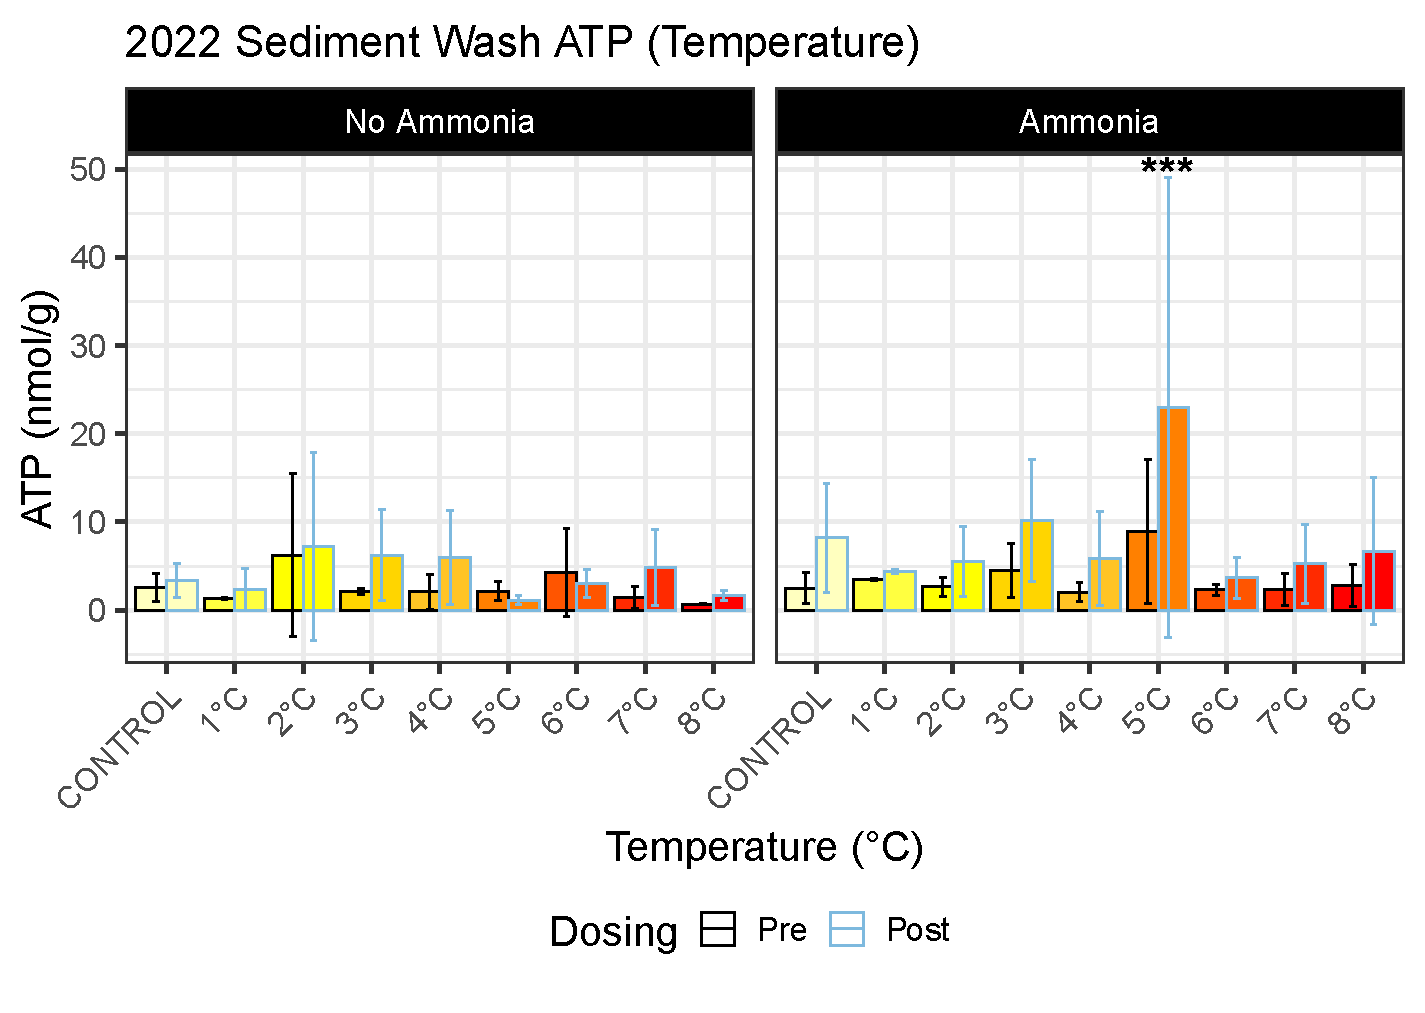
\includegraphics[scale=0.5]{./Figures/ATPSW2022_bar_temp}
    \caption{\textbf{Effects of gradient warming on microbial ATP production in 2022.} Half of the 96 ponds were treated with ammonia. 5°C warming significantly increased ATP production.}
    \label{fig:ATPSW2022_temp}
\end{figure}

\subsubsection{ATP production from sediment samples}

\begin{table}[H]
    \caption{{\bf The performance of LMM (p-values) in determining the effect of different chemical treatments on sediment ATP.} All treatments did not significantly affect ATP production. }
    \centering
    \begin{tabular}{ m{2.5cm}<{\centering}m{1.5cm}<{\centering}m{1.5cm}<{\centering}m{1.5cm}<{\centering}m{1.5cm}<{\centering}m{2.2cm}<{\centering}m{2.2cm}<{\centering}}
    \toprule
    Treatment & 4°C & UR & RU & UR+RU & UR+RU+4°C & Temperature \\
     \midrule
    No Ammonia & 0.517 & 0.627 & 0.419 & 0.216 & 0.700 & 0.390 \\
    Ammonia & 0.595 & 0.990 & 0.684 & 0.703 & 0.720 & 0.115 \\
    \bottomrule
    \end{tabular}    
    \label{tab:ATPS_treat}
\end{table}

\begin{table}[H]
    \caption{{\bf The performance of LMM (p-values and effect sizes) in determining the effect of different temperature treatments on 2022 sediment ATP.} Where p-values are \textless 0.05, they are shown in bold and the effect size (Cohen's d) is in the corresponding parentheses below. Only 8°C warming in ammonia-treated ponds significantly increased ATP production.}
    \centering
    \begin{tabular}{ m{2.5cm}<{\centering}m{1.2cm}<{\centering}m{1.2cm}<{\centering}m{1.2cm}<{\centering}m{1.2cm}<{\centering}m{1.2cm}<{\centering}m{1.2cm}<{\centering}m{1.2cm}<{\centering}m{1.2cm}<{\centering}} 
    \toprule
    Treatment & 1°C & 2°C & 3°C & 4°C & 5°C & 6°C & 7°C & 8°C \\
     \midrule
    No Ammonia & 0.319 & 0.095 & 0.740 & 0.517 & 0.840 & 0.577 & 0.718 & 0.326 \\
    \multirow{2}*{Ammonia} & 0.405 & 0.223 & 0.926 & 0.595 & 0.098 & 0.870 & 0.544 & \textbf{0.005} \\
     &  &  &  &  &  &  &  & (0.95) \\
    \bottomrule
    \end{tabular}    
    \label{tab:ATPS_temp}
\end{table}

\begin{figure}[H]
    \centering
    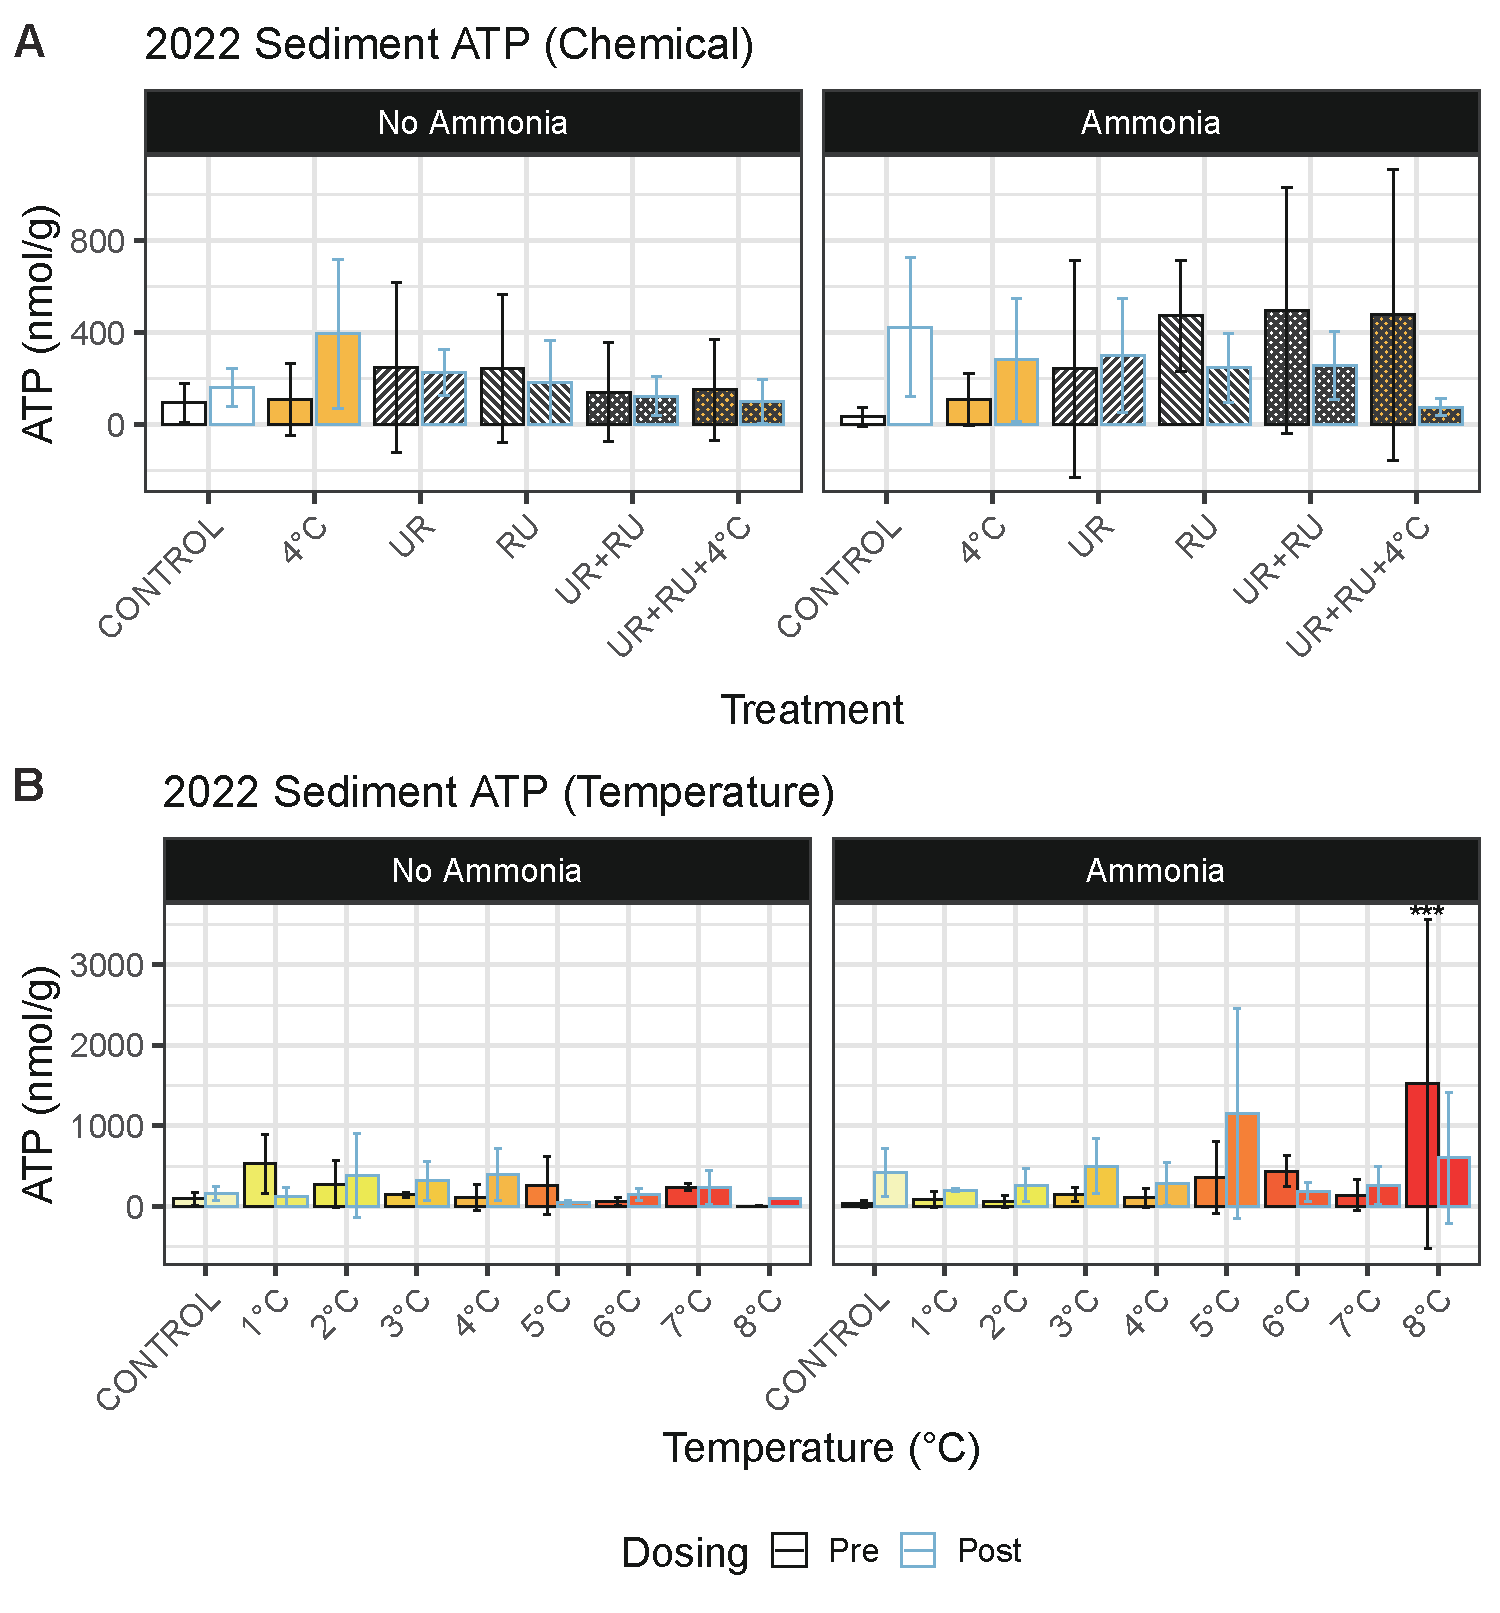
\includegraphics[scale=0.5]{./Figures/ATPS2022_bar}
    \caption{\textbf{Effects of chemical and gradient warming treatment on sediment microbial ATP production in 2022.} Biocides had an opposite effect on ATP production without and with ammonia treatment. The biocide significantly reduced ATP production through a synergistic effect with warming. In the ammonia-treated ponds, both 5 and 8°C warming significantly increased ATP production (which may be related to the abundance of biomass in ponds G11 and F7 respectively).}
    \label{fig:ATPS2022_bar}
\end{figure}

\subsubsection{ATP production from water samples}

\begin{table}[H]
    \caption{{\bf The performance of LMM (p-values and effect sizes) in determining the effect of different chemical treatments on water ATP.} Where p-values are \textless 0.05, they are shown in bold and the effect size (Cohen's d) is in the corresponding parentheses below. Only in the ammonia-treated ponds did gradient warming significantly increase the ATP production of the water samples.}
    \centering
    \begin{tabular}{ m{2.5cm}<{\centering}m{1.5cm}<{\centering}m{1.5cm}<{\centering}m{1.5cm}<{\centering}m{1.5cm}<{\centering}m{2.2cm}<{\centering}m{2.2cm}<{\centering}}
    \toprule
    Treatment & 4°C & UR & RU & UR+RU & UR+RU+4°C & Temperature \\
     \midrule
    No Ammonia & 0.133 & 0.468 & 0.735 & 0.872 & 0.209 & 0.646 \\
    \multirow{2}*{Ammonia} & 0.741 & 0.812 & 0.757 & 0.765 & 0.907 & \textbf{0.039} \\
     &  &  &  &  &  & (0.58) \\
    \bottomrule
    \end{tabular}    
    \label{tab:ATPW_treat}
\end{table}

\begin{table}[H]
    \caption{{\bf The performance of LMM (p-values and effect sizes) in determining the effect of different temperature treatments on 2022 water ATP.} Where p-values are \textless 0.05, they are shown in bold and the effect size (Cohen's d) is in the corresponding parentheses below. Under ammonia treatment, an 8°C warming significantly increased ATP production.}
    \centering
    \begin{tabular}{ m{2.5cm}<{\centering}m{1.2cm}<{\centering}m{1.2cm}<{\centering}m{1.2cm}<{\centering}m{1.2cm}<{\centering}m{1.2cm}<{\centering}m{1.2cm}<{\centering}m{1.2cm}<{\centering}m{1.2cm}<{\centering}} 
    \toprule
    Treatment & 1°C & 2°C & 3°C & 4°C & 5°C & 6°C & 7°C & 8°C \\
     \midrule
    No Ammonia & 0.129 & 0.11 & 0.649 & 0.133 & 0.776 & 0.711 & 0.179 & 0.871 \\
    \multirow{2}*{Ammonia} & 0.710 & 0.994 & 0.670 & 0.742 & 0.437 & 0.986 & 0.919 & \textbf{\textless 0.001} \\
     &  &  &  &  &  &  &  & (1.37) \\
    \bottomrule
    \end{tabular}    
    \label{tab:ATPW_temp}
\end{table}

\begin{figure}[H]
    \centering
    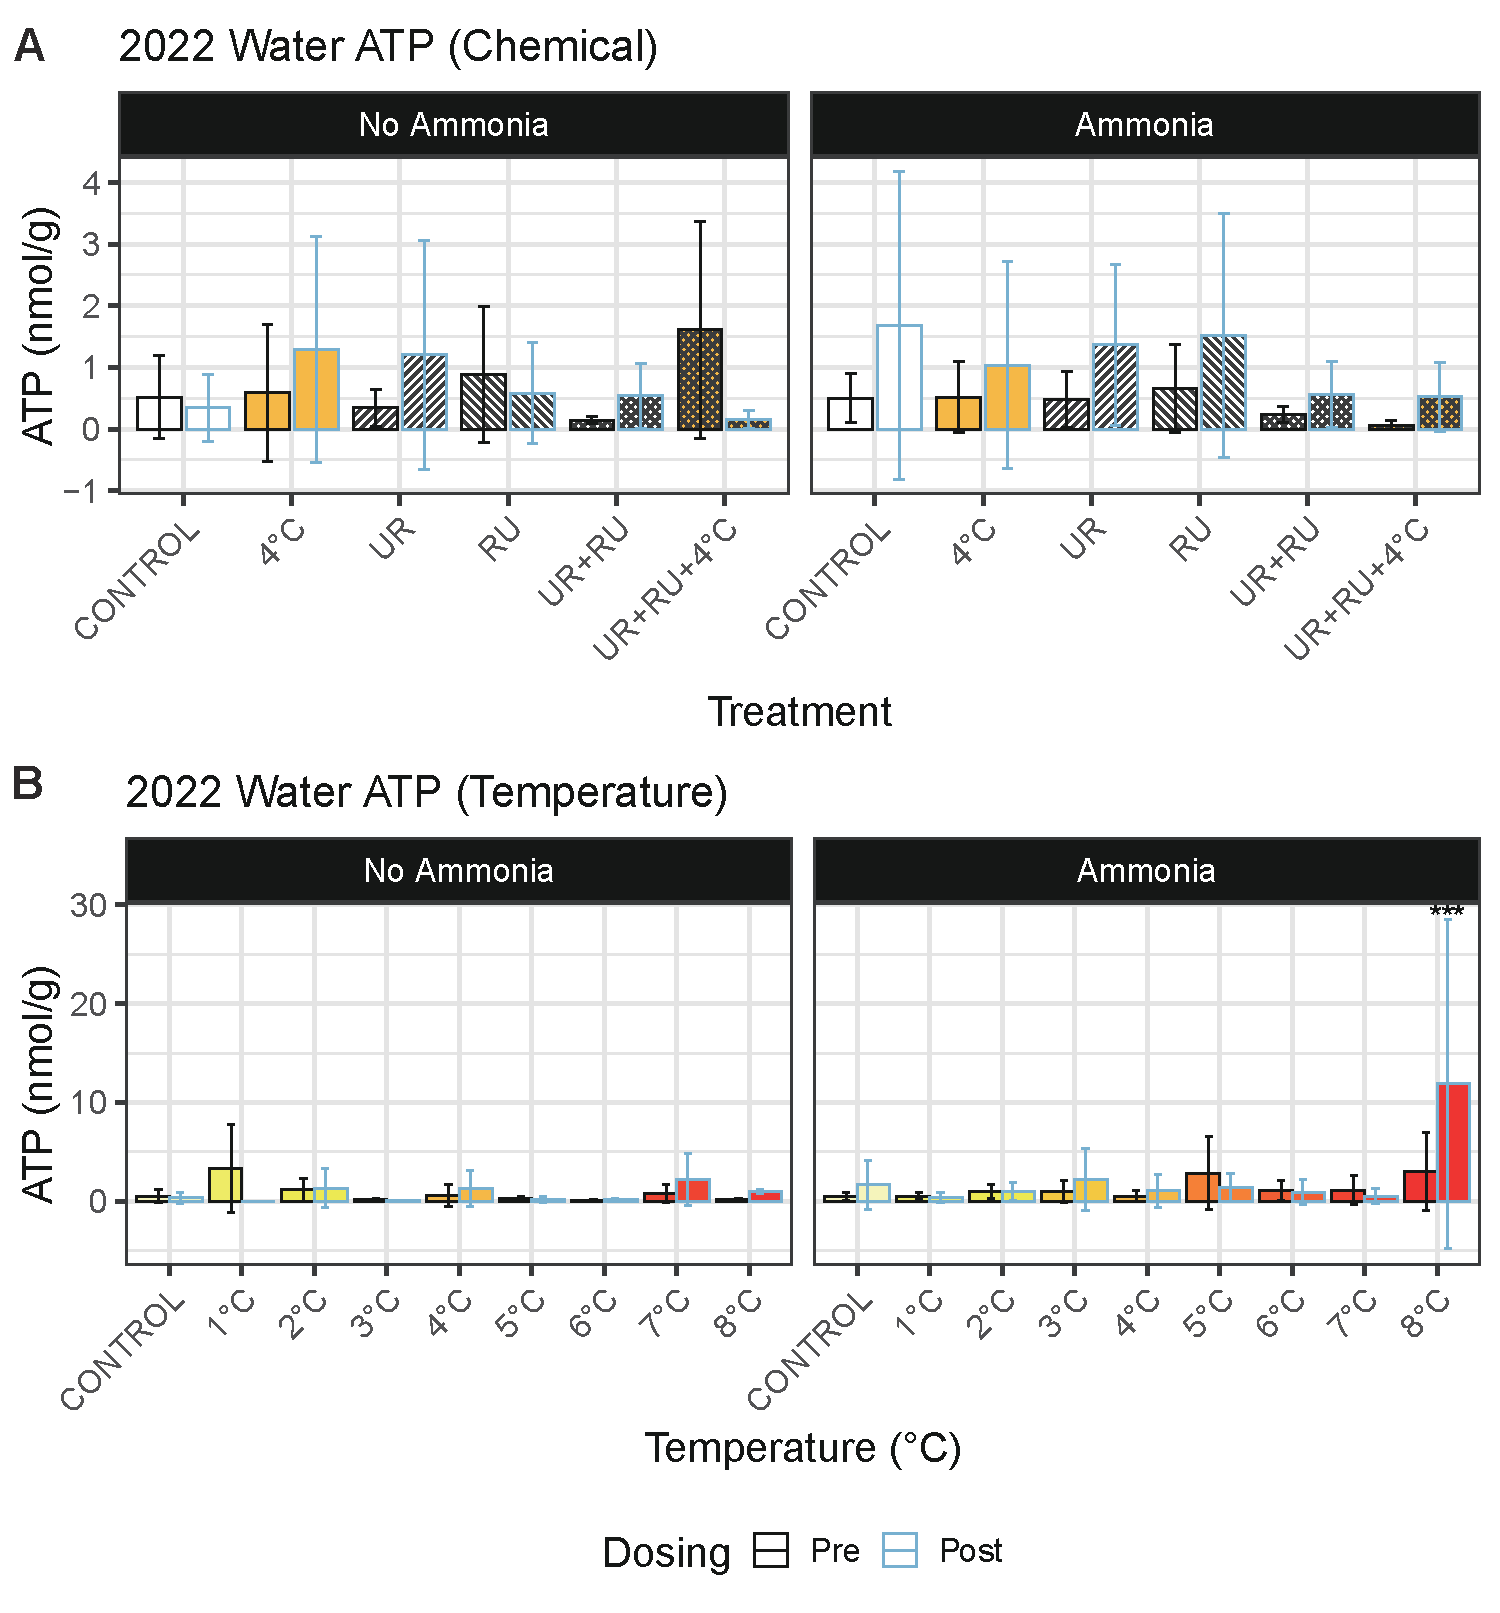
\includegraphics[scale=0.5]{./Figures/ATPW2022_bar}
    \caption{\textbf{Effects of chemical and gradient warming treatment on water microbial ATP production in 2022.} Biocides had an opposite effect on ATP production without and with ammonia treatment. The biocide significantly reduced ATP production through a synergistic effect with warming. In the ammonia-treated ponds, only 8°C warming significantly increased ATP production (which may be also related to the abundance of biomass in F7 pond).}
    \label{fig:ATPW2022_cp}
\end{figure}

\begin{table}[H]
    \caption{{\bf The performance of LMM (p-values and effect sizes) in determining the effect of different chemical treatments on water ATP (per-cell).} All treatments did not significantly affect ATP production.}
    \centering
    \begin{tabular}{ m{2.5cm}<{\centering}m{1.5cm}<{\centering}m{1.5cm}<{\centering}m{1.5cm}<{\centering}m{1.5cm}<{\centering}m{2.2cm}<{\centering}m{2.2cm}<{\centering}}
    \toprule
    Treatment & 4°C & UR & RU & UR+RU & UR+RU+4°C & Temperature \\
     \midrule
    No Ammonia & 0.208 & 0.989 & 0.803 & 0.989 & 0.482 & 0.702 \\
    Ammonia & 0.258 & 0.125 & 0.127 & 0.394 & 0.611 & 0.854 \\
    \bottomrule
    \end{tabular}    
    \label{tab:ATPpc_treat}
\end{table}

\begin{table}[H]
    \caption{{\bf The performance of LMM (p-values and effect sizes) in determining the effect of different temperature treatments on 2022 water ATP (per-cell).} Where p-values are \textless 0.05, they are shown in bold and the effect size (Cohen's d) is in the corresponding parentheses below. Only 1°C warming significantly increased ATP production.}
    \centering
    \begin{tabular}{ m{2.5cm}<{\centering}m{1.2cm}<{\centering}m{1.2cm}<{\centering}m{1.2cm}<{\centering}m{1.2cm}<{\centering}m{1.2cm}<{\centering}m{1.2cm}<{\centering}m{1.2cm}<{\centering}m{1.2cm}<{\centering}} 
    \toprule
    Treatment & 1°C & 2°C & 3°C & 4°C & 5°C & 6°C & 7°C & 8°C \\
     \midrule
    \multirow{2}*{No Ammonia} & \textbf{0.029} & 0.198 & 0.732 & 0.208 & 0.791 & 0.795 & 0.939 & 0.968 \\
     & (0.49) &  &  &  &  &  &  &  \\
    Ammonia & 0.617 & 0.207 & 0.396 & 0.258 & 0.633 & 0.618 & 0.774 & 0.418 \\
    \bottomrule
    \end{tabular}    
    \label{tab:ATPpc_temp}
\end{table}

\begin{figure}[H]
    \centering
    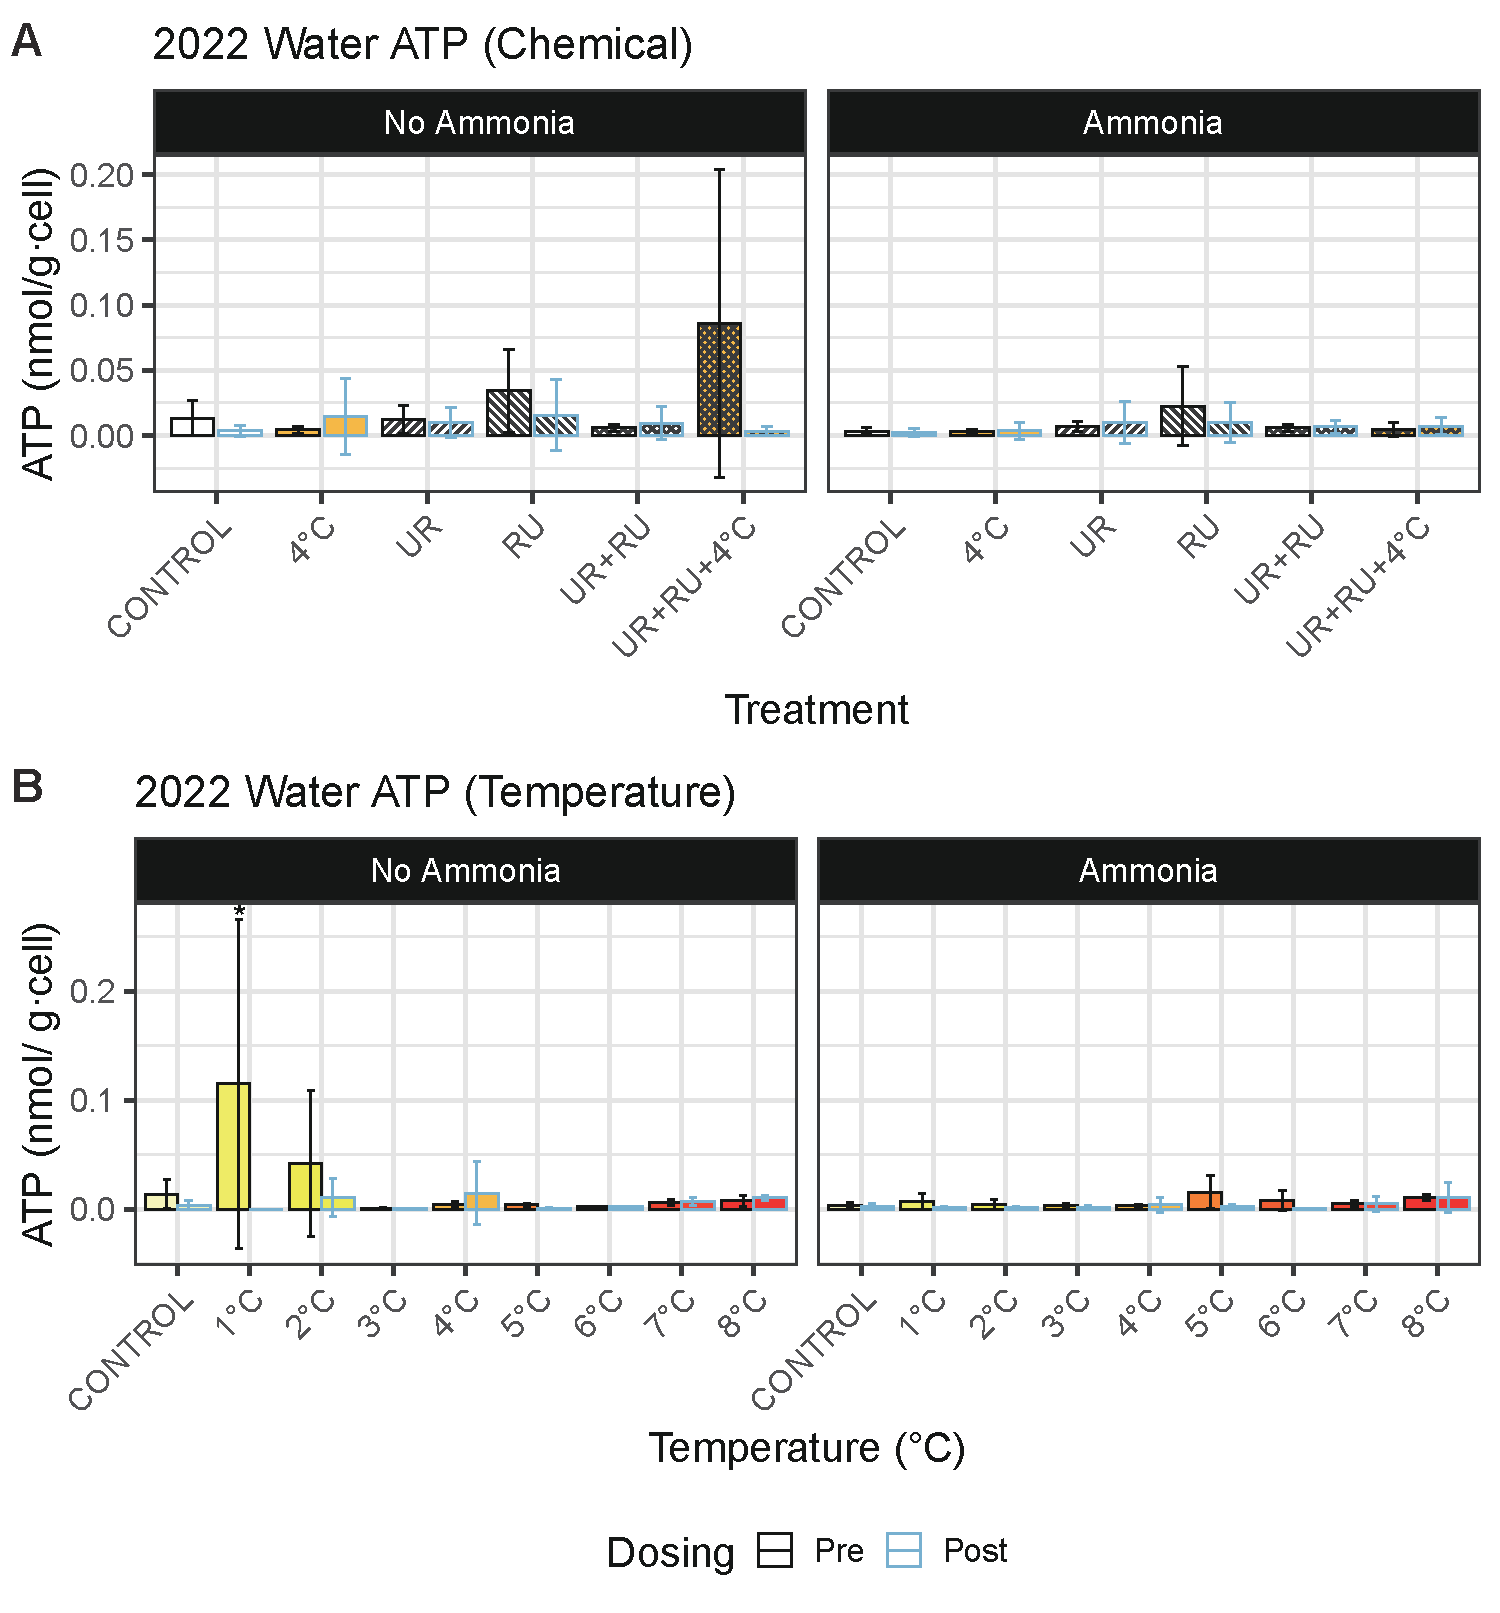
\includegraphics[scale=0.5]{./Figures/ATPWpc2022_bar}
    \caption{\textbf{Effects of chemical and gradient warming treatment on cell microbial ATP production of water samples in 2022.} Only 1°C warming significantly increased ATP production (which may be related to the B1 pond).}
    \label{fig:ATPpc2022_cp}
\end{figure}

\subsection{MicroResp}\label{section:MRS}

\begin{table}[H]
    \caption{{\bf The performance of LMM (p-values and effect sizes) in determining the effect of different chemical treatments on sediment wash MicroResp.} All treatments did not significantly affect microbial respiration.}
    \centering
    \begin{tabular}{ m{2.5cm}<{\centering}m{1.5cm}<{\centering}m{1.5cm}<{\centering}m{1.5cm}<{\centering}m{1.5cm}<{\centering}m{2.2cm}<{\centering}m{2.2cm}<{\centering}}
    \toprule
    Treatment & 4°C & UR & RU & UR+RU & UR+RU+4°C & Temperature \\
     \midrule
    No Ammonia & 0.690 & 0.564 & 0.275 & 0.136 & 0.537 & 0.412 \\
    Ammonia & 0.956 & 0.476 & 0.718 & 0.921 & 0.191 & 0.544 \\
    \bottomrule
    \end{tabular}    
    \label{tab:MR_treat}
\end{table}

\begin{table}[H]
    \caption{{\bf The performance of LMM (p-values and effect sizes) in determining the effect of different temperature treatments on 2022 sediment wash MicroResp.} All warming treatments did not significantly affect microbial respiration.}
    \centering
    \begin{tabular}{ m{2.5cm}<{\centering}m{1.2cm}<{\centering}m{1.2cm}<{\centering}m{1.2cm}<{\centering}m{1.2cm}<{\centering}m{1.2cm}<{\centering}m{1.2cm}<{\centering}m{1.2cm}<{\centering}m{1.2cm}<{\centering}} 
    \toprule
    Treatment & 1°C & 2°C & 3°C & 4°C & 5°C & 6°C & 7°C & 8°C \\
     \midrule
    No Ammonia & 0.500 & 0.501 & 0.739 & 0.690 & 0.491 & 0.263 & 0.211 & 0.068 \\
    Ammonia & 0.722 & 0.423 & 0.122 & 0.956 & 0.653 & 0.614 & 0.680 & 0.583 \\
    \bottomrule
    \end{tabular}    
    \label{tab:MR_temp}
\end{table}

In the warming-treatment ponds, all warming treatments did not significantly affect respiration (Table \ref{tab:MR_temp}).

\begin{figure}[H]
    \centering
    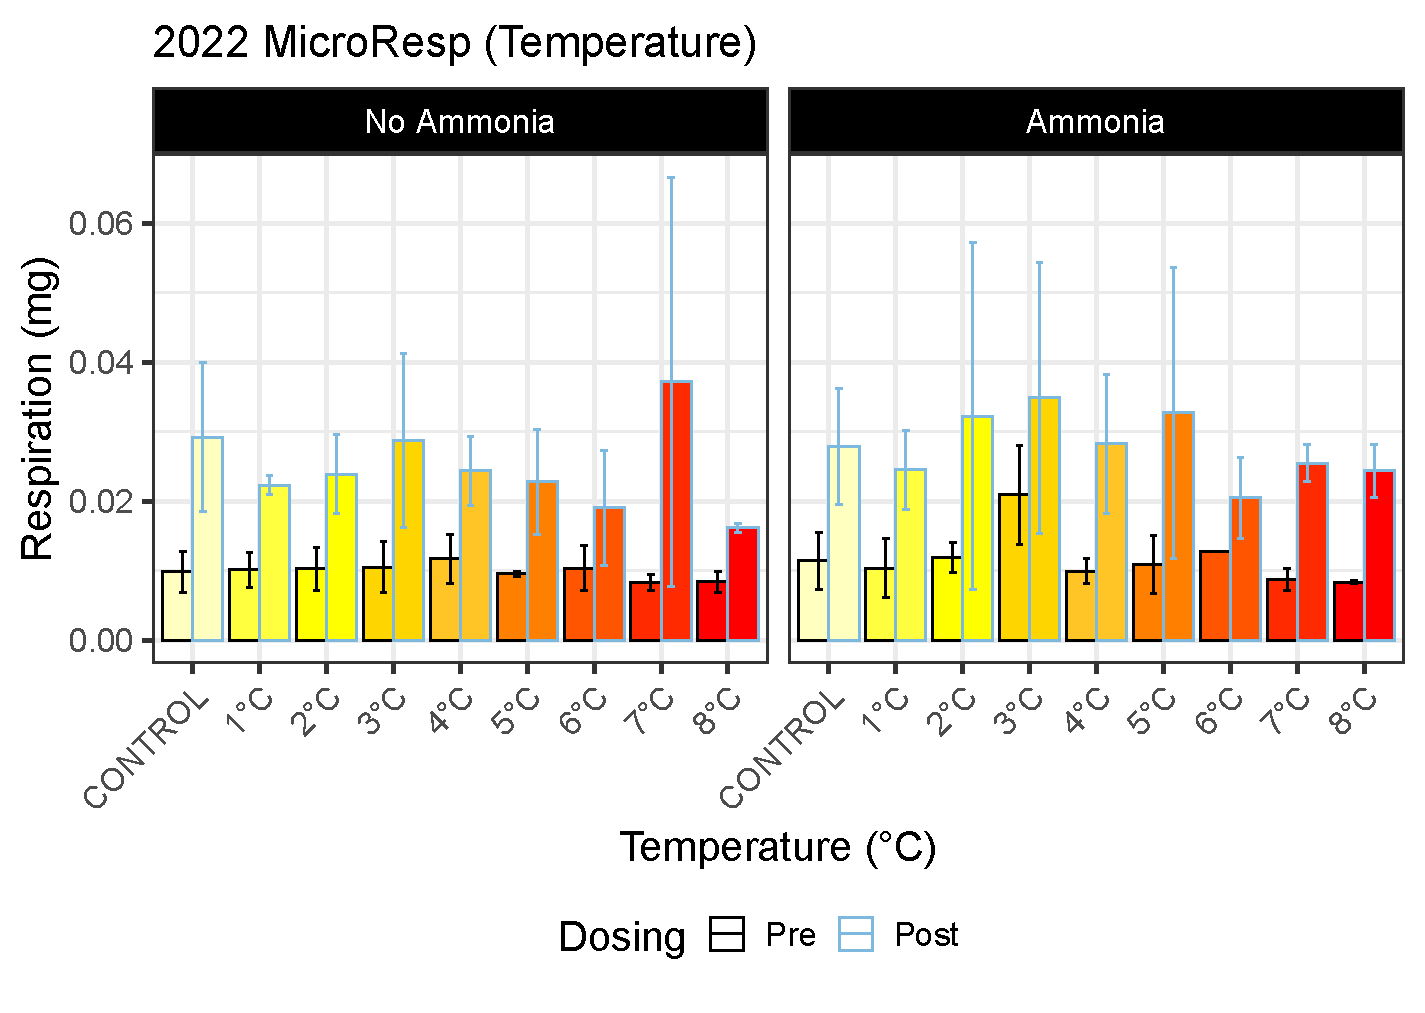
\includegraphics[scale=0.5]{./Figures/MicroResp2022_bar_temp}
    \caption{\textbf{Effects of gradient warming on microbial respiration in 2022.} Half of the 96 ponds were treated with ammonia. All warming treatments did not significantly affect microbial respiration.}
    \label{fig:MR2022_temp}
\end{figure}

\subsection{BOD}\label{section:BODS}

\begin{table}[H]
    \caption{{\bf The performance of LMM (p-values and effect sizes) in determining the effect of different chemical treatments on biochemical oxygen demand.} Where p-values are \textless 0.05, they are shown in bold and the effect size (Cohen's d) is in the corresponding parentheses below. Only the urban chemicals group significantly reduced BOD in the ponds without ammonia treatment. Under ammonia treatment, the combination of all biocides significantly reduced BOD, while they were significantly antagonistic to warming.}
    \centering
    \begin{tabular}{ m{2.5cm}<{\centering}m{1.5cm}<{\centering}m{1.5cm}<{\centering}m{1.5cm}<{\centering}m{1.5cm}<{\centering}m{2.2cm}<{\centering}m{2.2cm}<{\centering}}
    \toprule
    Treatment & 4°C & UR & RU & UR+RU & UR+RU+4°C & Temperature \\
     \midrule
    \multirow{2}*{No Ammonia} & 0.213 & \textbf{0.032} & 0.066 & 0.643 & 0.169 & 0.275 \\
     &  & (-0.53) &  &  &  & \\
    \multirow{2}*{Ammonia} & 0.286 & 0.089 & 0.073 & \textbf{0.010} & \textbf{0.031} & 1.000 \\
     &  &  &  & (-0.72) & (0.60) & \\
    \bottomrule
    \end{tabular}    
    \label{tab:BOD_treat}
\end{table}

\begin{table}[H]
    \caption{{\bf The performance of LMM (p-values and effect sizes) in determining the effect of different temperature treatments on 2022 biochemical oxygen demand.} All warming treatments did not significantly affect microbial respiration.}
    \centering
    \begin{tabular}{ m{2.5cm}<{\centering}m{1.2cm}<{\centering}m{1.2cm}<{\centering}m{1.2cm}<{\centering}m{1.2cm}<{\centering}m{1.2cm}<{\centering}m{1.2cm}<{\centering}m{1.2cm}<{\centering}m{1.2cm}<{\centering}} 
    \toprule
    Treatment & 1°C & 2°C & 3°C & 4°C & 5°C & 6°C & 7°C & 8°C \\
     \midrule
    No Ammonia & 0.297 & 0.573 & 0.859 & 0.213 & 0.989 & 0.239 & 0.349 & 0.149 \\
    Ammonia & 0.598 & 0.104 & 0.510 & 0.286 & 0.561 & 0.461 & 0.911 & 0.746 \\
    \bottomrule
    \end{tabular}    
    \label{tab:BOD_temp}
\end{table}

\begin{figure}[H]
    \centering
    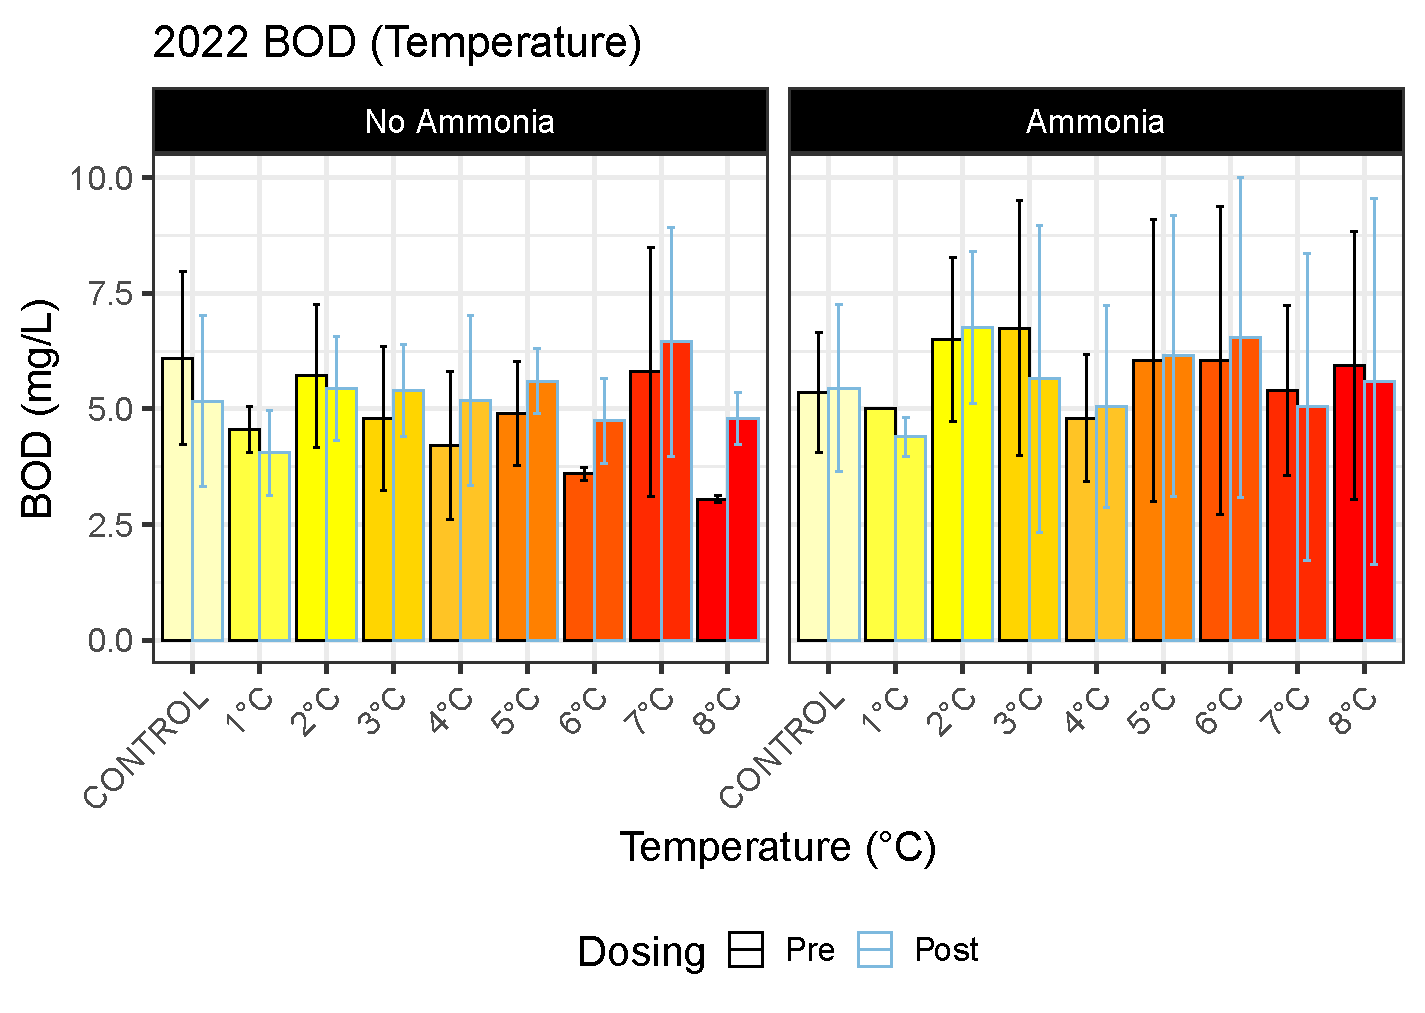
\includegraphics[scale=0.5]{./Figures/BOD2022_bar_temp}
    \caption{\textbf{Effects of gradient warming on biochemical oxygen demand in 2022.} Half of the 96 ponds were treated with ammonia. All warming treatments did not significantly affect BOD.}
    \label{fig:BOD2022_temp}
\end{figure}

\subsection{Tea bag decomposition}\label{section:TDS}

\begin{table}[H]
    \caption{{\bf The performance of LMM (p-values and effect sizes) in determining the effect of different chemical treatments on 2022 decomposition.} Ponds without (NA) and with (A) ammonia treatment are calculated separately and the results without (NC) and with (TC) temperature correction are shown. Where p-values are \textless 0.05, they are shown in bold and the effect size (Cohen's d) is in the corresponding parentheses below. UR represents the urban chemicals group and RU represents the rural chemicals group. After temperature correction, the effect sizes all increased, and all significantly affected tea bag decomposition rates were reduced, except for the combination of warming and the two chemial groups.}
    \centering
    \begin{tabular}{ m{2.2cm}<{\centering}m{1.2cm}<{\centering}m{1.2cm}<{\centering}m{1.2cm}<{\centering}m{1.2cm}<{\centering}m{1.2cm}<{\centering}m{1.2cm}<{\centering}m{1.2cm}<{\centering}m{1.2cm}<{\centering}} 
    \toprule
    & \multicolumn{2}{c}{Green (NA)} & \multicolumn{2}{c}{Rooibos (NA)} & \multicolumn{2}{c}{Green (A)} & \multicolumn{2}{c}{Rooibos (A)} \\
    Assay & NC & TC & NC & TC & NC & TC & NC & TC \\
     \midrule
    \multirow{2}*{4°C} & 0.133 & \textbf{\textless 0.001} & 0.061 & \textbf{\textless 0.001} & 0.095 & \textbf{\textless 0.001} & \textbf{0.019} & \textbf{\textless 0.001} \\
     &  & (-1.48) &  & (-1.49) &  & (-2.07) & (0.67) & (-1.80) \\
    \multirow{2}*{UR} & 0.641 & 0.977 & 0.424 & 0.896 & 0.065 & \textbf{0.010} & \textbf{0.039} & \textbf{0.037} \\
     &  &  &  &  &  & (-0.63) & (-0.46) & (-0.46) \\
    \multirow{2}*{RU} & 0.612 & 0.281 & 0.601 & 0.085 & 0.387 & \textbf{0.027} & \textbf{0.014} & 0.404 \\
     &  &  &  &  &  & (-0.54) & (0.55) &  \\
    \multirow{2}*{UR+RU} & 0.057 & \textbf{0.006} & 0.885 & 0.195 & 0.071 & \textbf{0.006} & 0.993 & 0.663 \\
     &  & (-0.63) &  &  &  & (-0.67) &  &  \\
    \multirow{2}*{UR+RU+4°C} & \textbf{0.011} & \textbf{\textless 0.001} & 0.735 & \textbf{0.015} & \textbf{0.011} & \textbf{0.001} & 0.886 & 0.568 \\
     & (0.61) & (0.99) &  & (0.58) & (0.66) & (0.83) &  &  \\
    \multirow{2}*{Temperature} & \textbf{\textless 0.001} & \textbf{\textless 0.001} & \textbf{\textless 0.001} & \textbf{\textless 0.001} & \textbf{0.007} & \textbf{\textless 0.001} & \textbf{0.015} & \textbf{\textless 0.001} \\
     & (1.01) & (-1.71) & (1.23) & (-1.85) & (0.79) & (-2.47) & (0.68) & (-2.67) \\
    \bottomrule
    \end{tabular}    
    \label{tab:D_2022chem}
\end{table}

In the temperature treatment ponds, 1, 2, 3, and 6°C of warming did not affect the decomposition rate (Table \ref{tab:D_2022temp}). All treatments that had significant effects on decomposition increased the decomposition rate. After correction for temperature, nearly all warming treatments significantly decreased the rate (Figure \ref{fig:Tea2022tcp}).

\begin{table}[H]
    \caption{{\bf The performance of LMM (p-values and effect sizes) in determining the effect of different temperature treatments on 2022 decomposition.} Ponds without (NA) and with (A) ammonia treatment are calculated separately and the results without (NC) and with (TC) temperature correction are shown. Where p-values are \textless 0.05, they are shown in bold and the effect size (Cohen's d) is in the corresponding parentheses below. After temperature correction, nearly all warming treatments significantly affected the tea bag decomposition and reduced the rate of decomposition.}
    \centering
    \begin{tabular}{ m{2.2cm}<{\centering}m{1.2cm}<{\centering}m{1.2cm}<{\centering}m{1.2cm}<{\centering}m{1.2cm}<{\centering}m{1.2cm}<{\centering}m{1.2cm}<{\centering}m{1.2cm}<{\centering}m{1.2cm}<{\centering}} 
    \toprule
    & \multicolumn{2}{c}{Green (NA)} & \multicolumn{2}{c}{Rooibos (NA)} & \multicolumn{2}{c}{Green (A)} & \multicolumn{2}{c}{Rooibos (A)} \\
    Assay & NC & TC & NC & TC & NC & TC & NC & TC \\
     \midrule
    \multirow{2}*{1°C} & 0.741 & 0.152 & 0.478 & 0.118 & 0.535 & \textbf{0.014} & 0.352 & \textbf{0.006} \\
     &  &  &  &  &  & (-0.86) &  & (-0.95) \\
    \multirow{2}*{2°C} & 0.274 & \textbf{0.022} & 0.313 & \textbf{0.017} & 0.499 & \textbf{\textless 0.001} & 0.914 & \textbf{\textless 0.001} \\
     &  & (-0.73) &  & (-0.80) &  & (-1.18) &  & (-1.29) \\
    \multirow{2}*{3°C} & 0.543 & \textbf{0.009} & 0.356 & 0.129 & 0.379 & \textbf{\textless 0.001} & 0.836 & \textbf{\textless 0.001} \\
     &  & (-0.89) &  &  &  &  (-1.60) &  & (-1.32) \\
    \multirow{2}*{4°C} & 0.133 & \textbf{\textless 0.001} & 0.061 & \textbf{\textless 0.001} & 0.095 & \textbf{\textless 0.001} & \textbf{0.019} & \textbf{\textless 0.001} \\
     &  & (-1.48) &  & (-1.49) &  & (-2.07) & (0.67) &  (-1.80) \\
    \multirow{2}*{5°C} & 0.078 & \textbf{0.028} & \textbf{0.038} & \textbf{0.041} & \textbf{0.014} & \textbf{0.002} & 0.059 & \textbf{\textless 0.001} \\
     &  & (-0.74) & (0.74) & (-0.73) & (0.85) & (-1.11) &  & (-1.27) \\
    \multirow{2}*{6°C} & 0.964 & \textbf{\textless 0.001} & 0.481 & \textbf{\textless 0.001} & 0.103 & \textbf{\textless 0.001} & 0.381 & \textbf{\textless 0.001} \\
     &  & (-1.27) &  & (-1.24) &  & (-1.42) &  &  (-1.65) \\
    \multirow{2}*{7°C} & 0.139 & \textbf{\textless 0.001} & \textbf{0.027} & \textbf{\textless 0.001} & 0.306 & \textbf{\textless 0.001} & 0.263 & \textbf{\textless 0.001} \\
     &  & (-1.36) & (0.79) & (-1.33) &  & (-1.89) &  & (-1.96) \\
    \multirow{2}*{8°C} & \textbf{\textless 0.001} & \textbf{0.013} & \textbf{0.001} & \textbf{0.001} & 0.186 & \textbf{\textless 0.001} & 0.535 & \textbf{\textless 0.001} \\
     & (1.49) & (-0.85) & (1.19) & (-1.19) &  & (-1.92) &  & (-2.19) \\
    \bottomrule
    \end{tabular}    
    \label{tab:D_2022temp}
\end{table}

\begin{figure}[H]
    \centering
    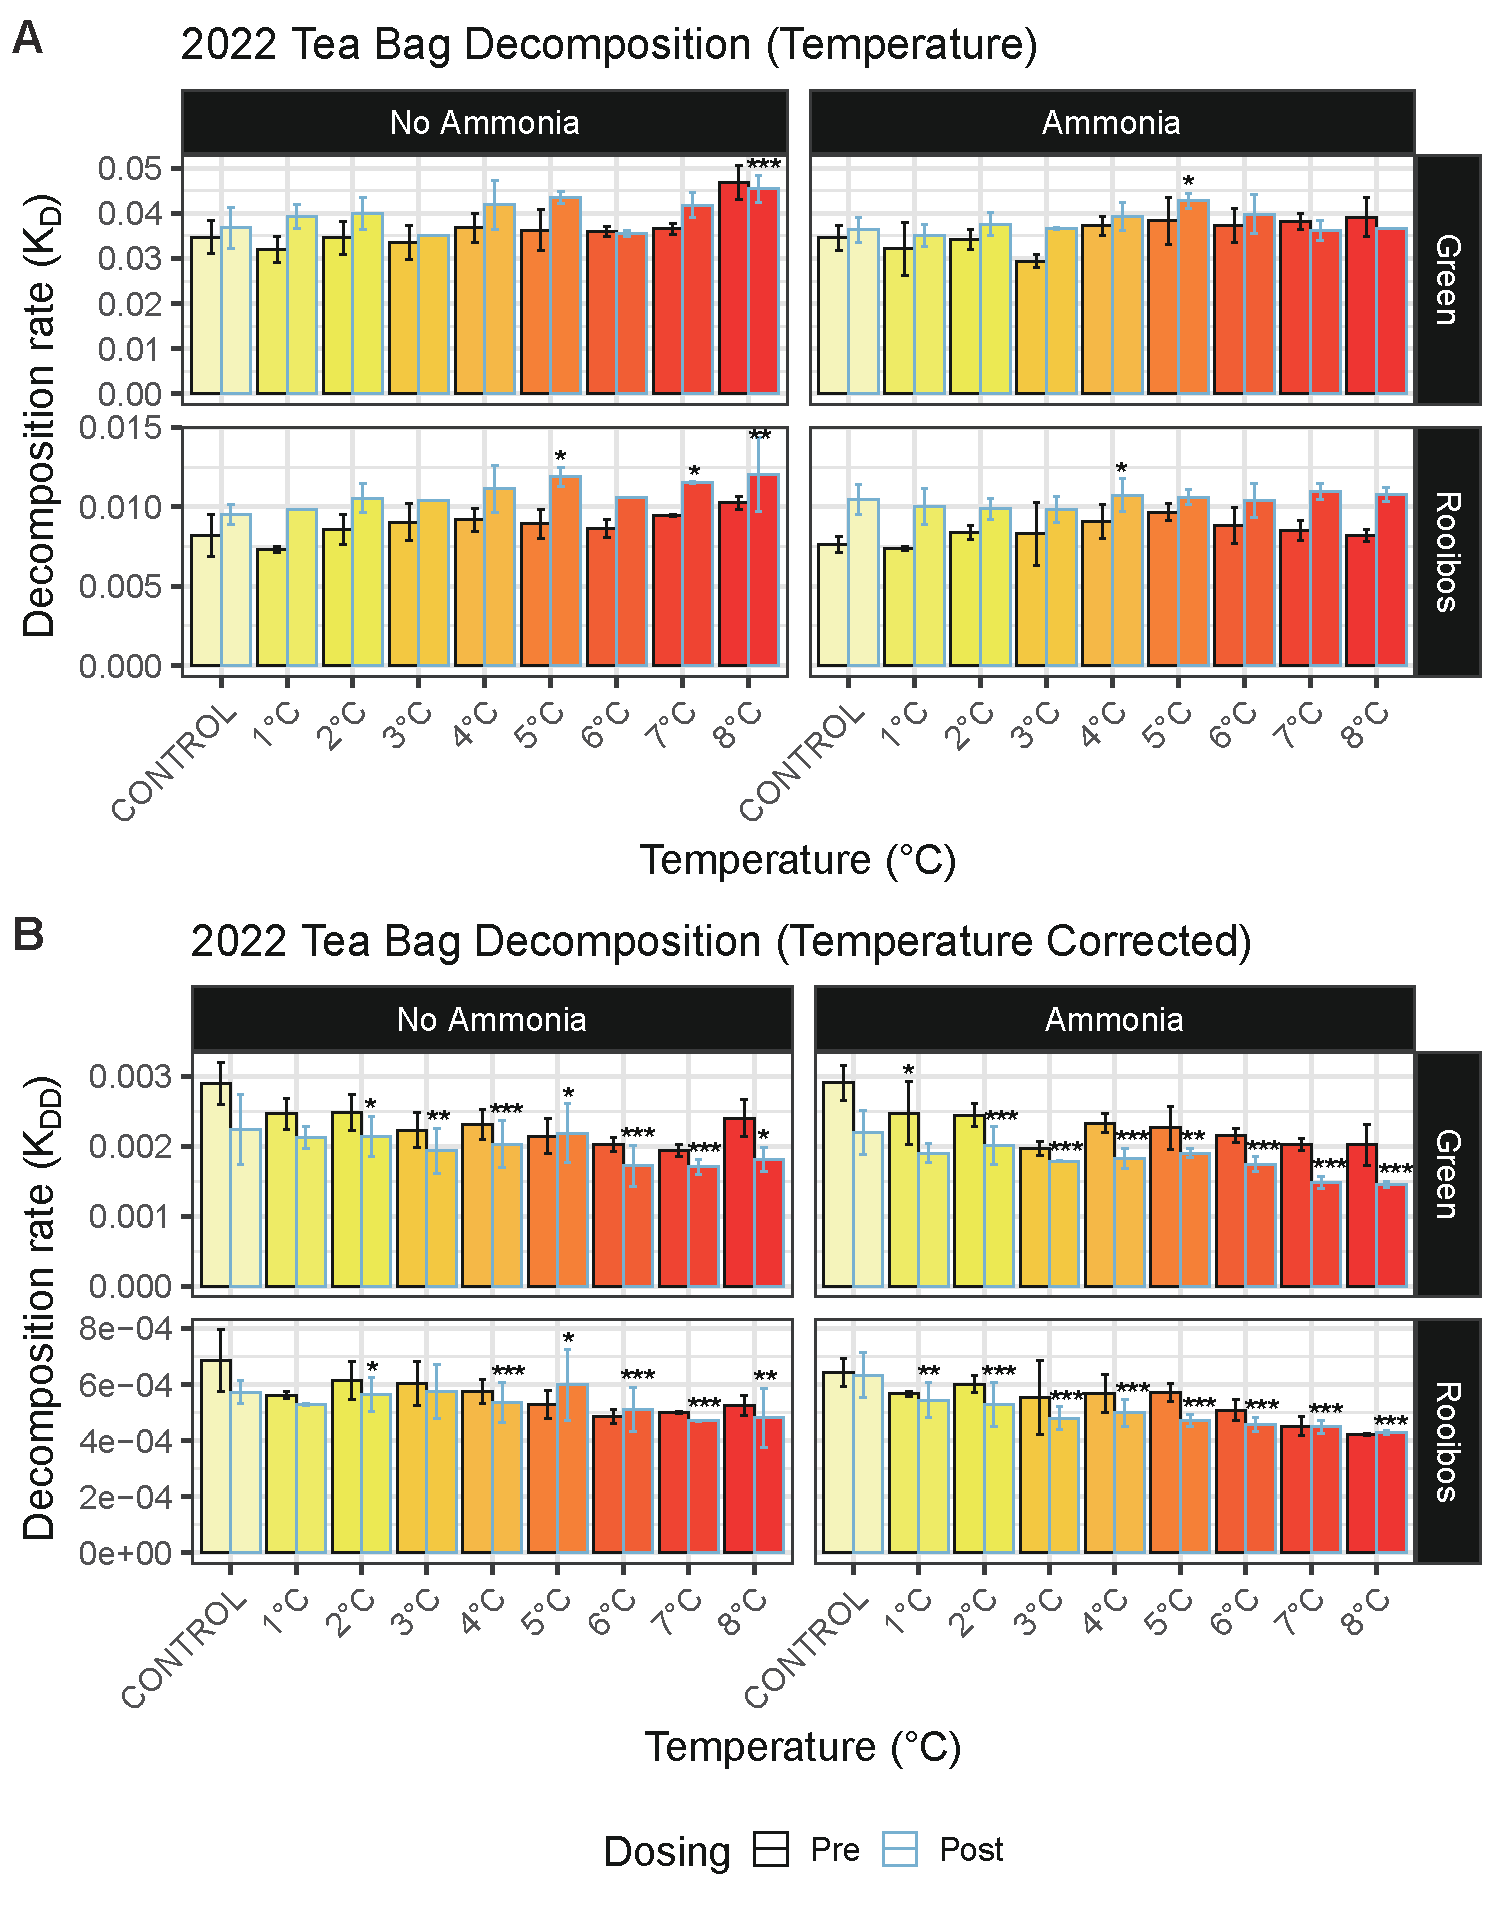
\includegraphics[scale=0.55]{./Figures/Tea2022_Temp_bar}
    \caption{\textbf{Effects of gradient warming on tea bag decomposition in 2022.} The tea bag decomposition rate increased with increasing temperature in the ponds without ammonia treatment, whereas the decomposition rate was minimally affected by temperature in the ammonia-treated ponds. After correction for temperature, decomposition rates decreased with increasing temperature.}
    \label{fig:Tea2022tcp}
\end{figure}

\subsection{Microbial functional assays in 2019-2022}\label{section:3YearS}

\subsubsection{ATP production}

\begin{table}[H]
    \caption{{\bf The performance of LMM (p-values and effect sizes) in determining the effect of different chemical treatments on 2019-2022 sediment wash ATP.} Where p-values are \textless 0.05, they are shown in bold and the effect size (Cohen's d) is in the corresponding parentheses below. Only the combination of the two chemical groups significantly reduced ATP.}
    \centering
    \begin{tabular}{ m{2.5cm}<{\centering}m{1.5cm}<{\centering}m{1.5cm}<{\centering}m{1.5cm}<{\centering}m{1.5cm}<{\centering}m{2.2cm}<{\centering}}
    \toprule
     & 4°C & UR & RU & UR+RU & UR+RU+4°C \\
     \midrule
    p-value & 0.803 & 0.925 & 0.458 & \textbf{0.044} & 0.963 \\
    Cohen's d &  &  &  & (-0.37) &  \\
    \bottomrule
    \end{tabular}    
    \label{tab:ATPSW_3Year}
\end{table}

\subsubsection{Microbial respiration}

\begin{table}[H]
    \caption{{\bf The performance of LMM (p-values and effect sizes) in determining the effect of different chemical treatments on 2019-2022 MicroResp.} Where p-values are \textless 0.05, they are shown in bold and the effect size (Cohen's d) is in the corresponding parentheses below. Both warming (4°C) and the combination of the two chemical groups significantly reduced microbial respiration.}
    \centering
    \begin{tabular}{ m{2.5cm}<{\centering}m{1.5cm}<{\centering}m{1.5cm}<{\centering}m{1.5cm}<{\centering}m{1.5cm}<{\centering}m{2.2cm}<{\centering}}
    \toprule
     & 4°C & UR & RU & UR+RU & UR+RU+4°C \\
     \midrule
    p-value & \textbf{0.040} & 0.636 & 0.441 & \textbf{0.050} & 0.140 \\
    Cohen's d & (-0.62) &  &  & (-0.59) &  \\
    \bottomrule
    \end{tabular}    
    \label{tab:MicroResp_3Year}
\end{table}

\subsubsection{Leaf decomposition}

\begin{table}[H]
    \caption{{\bf The performance of LMM (p-values and effect sizes) in determining the effect of different chemical treatments on 2019-2022 leaf decomposition.} The coarse and fine mesh leaf bags are calculated separately and the results without (NC) and with (TC) temperature correction are shown. Where p-values are \textless 0.05, they are shown in bold and the effect size (Cohen's d) is in the corresponding parentheses below. Only the warming (4°C) had significant effects on leaf decomposition.}
    \centering
    \begin{tabular}{ m{1.5cm}<{\centering}m{1.1cm}<{\centering}m{1.1cm}<{\centering}m{1cm}<{\centering}m{1cm}<{\centering}m{1.1cm}<{\centering}m{1.1cm}<{\centering}m{1cm}<{\centering}m{1cm}<{\centering}m{1cm}<{\centering}m{1cm}<{\centering}} 
    \toprule
    & \multicolumn{2}{c}{4°C} & \multicolumn{2}{c}{UR} & \multicolumn{2}{c}{RU} & \multicolumn{2}{c}{UR+RU} & \multicolumn{2}{c}{UR+RU+4°C} \\
    Assay & NC & TC & NC & TC & NC & TC & NC & TC & NC & TC \\
     \midrule
    \multirow{2}*{Coarse} & \textbf{\textless 0.001} & 0.436 & 0.906 & 0.976 & 0.327 & 0.525 & 1.000 & 0.794 & 0.216 & 0.543 \\
     & (0.78) &  &  &  &  &  &  &  &  &  \\
    \multirow{2}*{Fine} & \textbf{0.012} & \textbf{0.026} & 0.204 & 0.178 & 0.584 & 0.367 & 0.558 & 0.382 & 0.920 & 0.602 \\
     & (0.68) & (-0.60) &  &  &  &  &  &  &  &  \\
    \bottomrule
    \end{tabular}    
    \label{tab:LD_3Year}
\end{table}

\subsection{Flow cytometer}\label{section:Flow}

\begin{figure}[H]
    \centering
    \includegraphics[scale=0.6]{./Figures/20220420_1_6}
    \caption{\textbf{Cell counts in water samples from all ponds numbered 1-6 before dosing in 2022.} A07.fcs is the control.}
    \label{fig:fc2022_pre_1_6}
\end{figure}

\begin{figure}[H]
    \centering
    \includegraphics[scale=0.6]{./Figures/20220420_7_12}
    \caption{\textbf{Cell counts in water samples from all ponds numbered 7-12 before dosing in 2022.} A06.fcs is the control.}
    \label{fig:fc2022_pre_7_12}
\end{figure}

\begin{figure}[H]
    \centering
    \includegraphics[scale=0.6]{./Figures/20220517_1_6}
    \caption{\textbf{Cell counts in water samples from all ponds numbered 1-6 after dosing in 2022.} A07.fcs is the control.}
    \label{fig:fc2022_post_1_6}
\end{figure}

\begin{figure}[H]
    \centering
    \includegraphics[scale=0.6]{./Figures/20220517_7_12}
    \caption{\textbf{Cell counts in water samples from all ponds numbered 7-12 after dosing in 2022.} A06.fcs is the control.}
    \label{fig:fc2022_post_7_12}
\end{figure}

\subsection{Enzyme assays}\label{section:Enzyme}

The metabolic activity of freshwater microbial communities was investigated by analyzing four enzymes (Table \ref{tab:Enzyme}). In this study, microbial extracellular enzyme activity was evaluated using several fluorescent substrates, each designed to target the enzyme to be examined precisely. Added 75$\upmu$l of fluorescent labelled substrate working solution to each well of a 96-well plate. Water, sediment wash, and a 1:10 dilution of the sediment were mixed well with the working solution in a deep well plate, and 25$\upmu$l was pipetted into a white 96 well plate containing the substrate. Incubated for 1h at 20°C (room temperature) in the dark, and then added 10$\upmu$l of 1M NaOH to stop the enzyme reaction. The plate was then placed in the BioTek$^\circledR$ Synergy 2 Multi-Detection Microplate Reader, and the fluorescence of each well was read at 1 minute intervals for 3 minutes, and the maximum fluorescence value was taken. Only comparisons of 2019 and 2021 enzyme data are available as the enzyme analysis was removed after the 2022 dosing, which can be found at my github "EECSummerProject"  (\href{https://github.com/ChuxuanJi/EECSummerProject/tree/master/Sandbox}{\color{blue}{\underline{Sandbox}}}) repository.

\begin{table}[H]
    \caption{\bf The extracellular enzymes measured, the substrates selected and the functions measured in the current study.}
    \centering
    \begin{tabular}{ |m{4.9cm}<{\centering}|m{6.3cm}<{\centering}|m{4.7cm}<{\centering}| } 
    \hline
     Enzyme Assayed & Substrate & General Function \\
     \hline
     Glucosidase & 4-MUB-D-glucopyranoside & Sugar degradation \\ 
     $\upbeta$-Xylosidase & 4-MUB-$\upbeta$-D-xylopyranoside & Hemicellulose degradation \\
     $\upbeta$-D-cellubiosidase & 4-MUB-$\upbeta$-D-cellobioside & Cellulose degradation \\
     N-acetyl-$\upbeta$-Glucosaminidase & 4-MUB-N-acetyl-$\upbeta$-D-glucosaminide & Chitin degradation \\
    \hline
    \end{tabular}    
    \label{tab:Enzyme}
\end{table}

\subsection{Wettex$^\circledR$ decomposition}\label{section:Wettex}

Due to the high variability of leaves, the decomposition rates of leaves of different individuals of the same tree species are different \citep{irons1991effects,sariyildiz2003decomposition,coleman2020leaf}, and the use of pure cellulose medium as a substrate would be more consistent. Determining Wettex$^\circledR$ sponge cloth decomposition rate is a standardised and inexpensive method of organic material determination for microbial decay analysis \citep{eriksen2022effects}. Wettex$^\circledR$ sponge cloth (Vileda$^\circledR$, EAN: 4 023103 118355)is biodegradable and made from renewable fibres, including 70\% cellulose and 30\% cotton. As with leaves, two kinds of mesh bags containing four pieces of Wettex$^\circledR$ (2.5 × 8.5 cm) were placed in mesocosms and cultured for 32 days. The drying and weighing steps were repeated, and the decomposition rate was calculated.

Unfortunately, the presence of worms and Gammaridea species in some of the fine mesh bags resulted in a final result that was not biologically significant. Therefore the decomposition data of Wettex$^\circledR$ were discarded in this study and its raw data can be found at my github "EECSummerProject"  (\href{https://github.com/ChuxuanJi/EECSummerProject/tree/master/Sandbox}{\color{blue}{\underline{Sandbox}}}) repository.

\end{document}